%% BoundingBox: 0 0 30 30
\documentclass[12pt]{article}
\usepackage{graphicx}
\usepackage{hyperref}
\usepackage{tabularx}
\usepackage[utf8]{inputenc}
\usepackage[english]{babel}
\pagestyle{plain}

\setcounter{secnumdepth}{2}
\graphicspath{{img/}}
\topmargin=0cm
\oddsidemargin=0cm
\textheight=22.0cm
\textwidth=16cm
\parindent=0cm
\parskip=0.15cm
\topskip=0truecm
\raggedbottom
\abovedisplayskip=3mm
\belowdisplayskip=3mm
\abovedisplayshortskip=0mm
\belowdisplayshortskip=2mm
\normalbaselineskip=12pt
\normalbaselines

\begin{document}

\vspace*{0.5in}
\centerline{\bf\Large Requirements Document}

\vspace*{0.5in}
\centerline{\bf\Large Team PI-b}

\vspace*{0.5in}
\centerline{\bf\Large 17 January 2019}

\vspace*{1.5in}
\begin{table}[htbp]
\caption{Team}
\begin{center}
\begin{tabular}{|r | c|}
\hline
Name & ID Number \\
\hline\hline
Max Page-Slowik & 40053948 \\
\hline
Simon Huang & 27067380 \\
\hline
Jonathan Massabni & 26337430 \\
\hline
Alexia Soucy & 40014822 \\
\hline
Anthony Funiciello& 40054110\\
\hline
    David Gray&40055149\\
\hline
Mair Elbaz&40004558\\
\hline
Rani Rafid&26975852\\
\hline
\end{tabular}
\end{center}
\end{table}

\clearpage

\section{System}

\subsection{Purpose}
Develop a working computer game based on the table top card game Codenames.
\subsection{Context}
The game is written in Java using the Java FX framework and will run as a desktop application. This will be a single user experience with only the person at the machine interacting with the device will be the user. The rest will be ran by the system.
\subsection{Business Goals}
To make a free and enjoyable experience with a quality user interface.
\section{Domain Concepts}
The domain we are working in is of the table top board game genre.\\
Therefore we are working with the concepts of cards, players, turns, a winner and a loser.\\
The games basis is to start with a board with a 5x5 grid of cards with nouns on them. The SpyMasters have a matching card that acts as the key cards showing the words they want their given operatives to pick. The SpyMaster does that by giving a hint consisting of a single noun and a number. The Operative then has that many guesses to find the hint that the SpyMaster has given per round. The SpyMaster places down the appropriate card for the given guess, if it is a bystander or the other team's colour it ends the turn, if it is the assassin it is game over and the other team wins, if it is all of the colours that given team wins when they are out of their colour. This game is played until the assassin is struck or all the colours are chosen for any given team.

\section{Actors}
\begin{enumerate}
\item User
\item Spy Master
\item Operative
\end{enumerate}
\newpage
\begin{figure}[htbp]
\centering
\includegraphics[width=16cm,height=14cm]{domain_model}
\caption{Domain Model}
\label{fig:domain-model-diagram}

\end{figure}
\newpage
\section{Use Cases}

\subsection{Overview}

% \begin{figure}[htbp]
% \centering
% \includegraphics[width=16cm,height=14cm]{use_case}
% \caption{Use Case Diagram}
% \label{fig:use-case}
% \end{figure}
% \newpage

\begin{figure}[htbp]
\centering
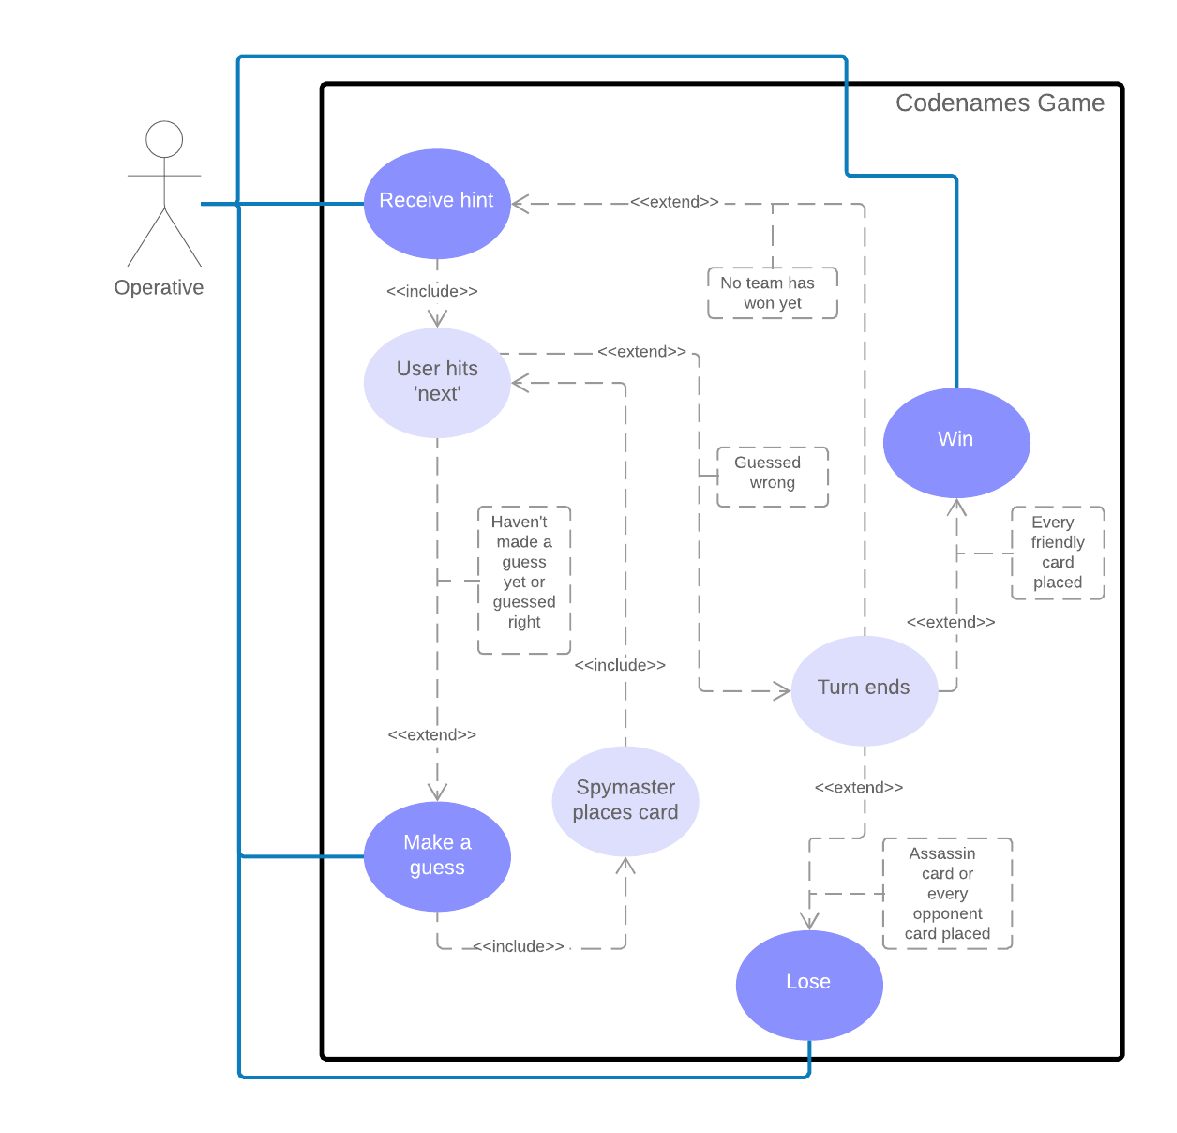
\includegraphics[width=16cm,height=14cm]{operative_ucd}
\caption{Use Case Operative Diagram}
\label{fig:use-case-operative}
\end{figure}
\newpage
\subsubsection{Use Case 1} \label{uc:1}

\noindent
{\bf Name}\\
Find noun

\noindent
{\bf Summary}\\
Based on the hint given, find the nouns that match on the board. Hint is Word, Number. the amount of guesses the Operator can make is Number + 1.

\noindent
{\bf Actors}\\
The Operative\\
\noindent
{\bf Precondition}\\
Hint given by the Spy Master\\
\noindent
{\bf Main Scenario}\\
\vspace*{-0.2in}
\begin{enumerate}
\item Pick a card on the board.
\end{enumerate}

\noindent
{\bf Exceptions}
\begin{enumerate}
\item If the Spy Master says 0 or infinity the Operative can make as many guesses as desired.
\item If the Operative decides not to guess. Goes to the other team colour Spy Master to start giving a hint.
\end{enumerate}

\noindent
{\bf Postcondition}\\
Give control back to the Spy Master to place the card or give control to other team to give a hint\\
\noindent
{\bf Priority}\\
Must have\\
\noindent
{\bf Traces to Test Cases}\\
Add when test cases done.

\newpage
\subsubsection{Use Case 2} \label{uc:2}

\noindent
{\bf Name}\\
Continue guessing

\noindent
{\bf Summary}\\
Based on the hint given, find the nouns that match on the board. The hint was given on the initial portion of the turn by the Spy Master. Each turn that is taken increases cannot exceed the Number + 1 that was given out in the initial hint.\\
\noindent
{\bf Actors}\\
The Operative\\
\noindent
{\bf Precondition}\\
Card was placed for your team colour by the Spy Master\\
\noindent
{\bf Main Scenario}\\
\vspace*{-0.2in}
\begin{enumerate}
\item Pick a card on the board.
\end{enumerate}

\noindent
{\bf Exceptions}
\begin{enumerate}
\item If the Spy Master says 0 or infinity the Operative can make as many guesses as desired.
\item If the Number + 1 total is reached then this is the last guess. Goes to the other Team colour Spy Master to start giving a hint.
\item If the Operative decides not to guess. Goes to the other Team colour Spy Master to start giving a hint.
\end{enumerate}
\noindent
{\bf Postcondition}\\
Give control back to the Spy Master to place the card or to the other team to give a hint\\
\noindent
{\bf Priority}\\
Good to have\\
\noindent
{\bf Traces to Test Cases}\\
Add when test cases done.
\newpage

\begin{figure}[htbp]
\centering
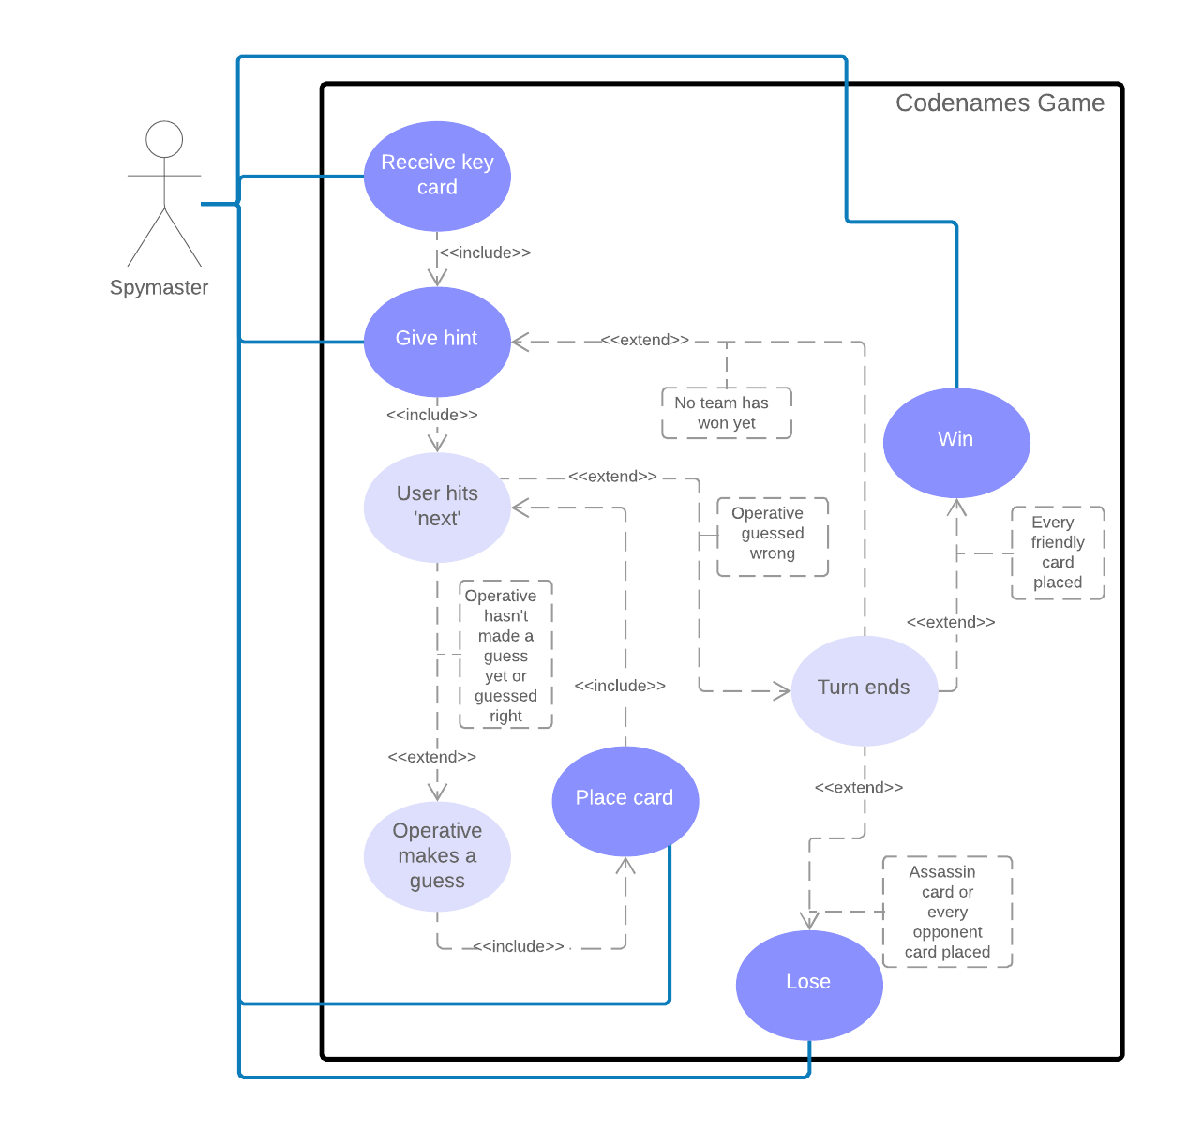
\includegraphics[width=16cm,height=14cm]{spymaster_ucd}
\caption{Use Case Spymaster Diagram}
\label{fig:use-case-spymaster}
\end{figure}
\newpage


\subsubsection{Use Case 3} \label{uc:3}

\noindent
{\bf Name}\\
Give a hint

\noindent
{\bf Summary}\\
hint consisting of one word and one number to be given to the operatives

\noindent
{\bf Primary Actors}\\
Spy masters\\
\noindent
{\bf Precondition}\\
Other team is out of guesses and it is your team's turn, or start of game\\
\noindent
{\bf Main Success Scenarios}\\
\vspace*{-0.2in}
\begin{enumerate}
\item Look at the remaining cards on the board
\item Say one noun
\item Say one number (0-infinity)
\end{enumerate}
\noindent
{\bf Exceptions}
\begin{enumerate}
\item if the noun is illegal, give another hint
\end{enumerate}
\noindent
{\bf Postcondition}\\
Give a hint that is insightful for your operatives\\
\noindent
{\bf Priority}\\
Must have\\
{\bf Traces to Test Cases}\\
Add when test cases done.
\noindent
\newpage

\subsubsection{Use Case 4} \label{uc:4}
\noindent
{\bf Name}\\
Place a card

\noindent
{\bf Summary}\\
Place a card on the board depending on the operatives' answers

\noindent
{\bf Primary Actors}\\
Spy masters\\
\noindent
{\bf Precondition}\\
The operative has selected a card on the board\\
\noindent
{\bf Main Success Scenarios}\\
\vspace*{-0.2in}
\begin{enumerate}
\item Listen to the operatives' guesses
\item Place the appropriate card
\item Give control back to the operative to make their next guess if any
\end{enumerate}
\noindent
{\bf Exceptions}
\begin{enumerate}
\item if guess lands on the other team's operatives, place their card and end the round
\item if guess lands on a civilian, place the card and end the round
\item if guess lands on the assassin, place the card and end the game
\item if out of guesses end the round and the next team colour starts
\end{enumerate}
\noindent
{\bf Postcondition}\\
Successfully place the appropriate card on the board\\
\noindent
{\bf Priority}\\
Good to have\\
\noindent
{\bf Traces to Test Cases}\\
Add when test cases done.
\newpage
\begin{figure}[htbp]
\centering
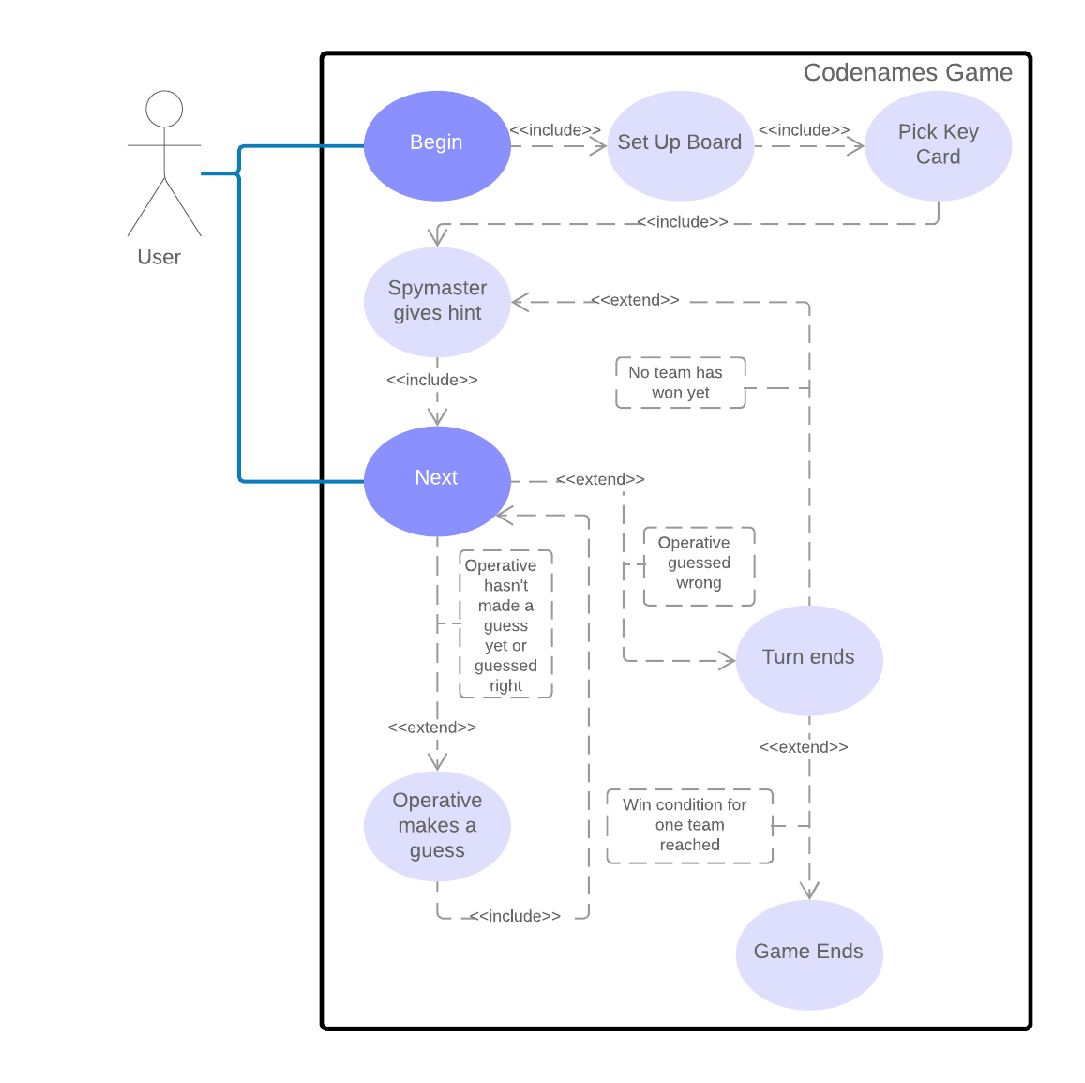
\includegraphics[width=16cm,height=14cm]{user_ucd}
\caption{Use Case User Diagram}
\label{fig:use-case-user}
\end{figure}
\newpage
\subsubsection{Use Case 5} \label{uc:5}
\noindent
{\bf Name}\\
Start the Game

\noindent
{\bf Summary}\\
User clicks begin to start the game

\noindent
{\bf Primary Actors}\\
Users\\
\noindent
{\bf Precondition}\\
The game must successfully load and display a "start" button

\noindent
{\bf Main Success Scenarios}\\
\vspace*{-0.2in}
\begin{enumerate}
\item Click on "start"
\item display the board
\item display who is the first team to start
\end{enumerate}
\noindent
{\bf Exceptions}
\begin{enumerate}
\item if the game doesn't load, display an error message
\end{enumerate}
\noindent
{\bf Postcondition}\\
The game is successfully initiated and the board displayed\\
\noindent
{\bf Priority}\\
Must have\\
\noindent
{\bf Traces to Test Cases}\\
Add when test cases done.
\newpage

\subsubsection{Use Case 6} \label{uc:6}
\noindent
{\bf Name}\\
Click "next"

\noindent
{\bf Summary}\\
User clicks "next" to simulate the game until the program ends

\noindent
{\bf Primary Actors}\\
Users\\
\noindent
{\bf Precondition}\\
The game must have successfully started and a "next" button is displayed

\noindent
{\bf Main Success Scenarios}\\
\vspace*{-0.2in}
\begin{enumerate}
\item Click on "next"
\item Display the next simulated move
\item Display the winner of the game: red or blue team
\item Terminate and display a "new game" option 
\end{enumerate}
\noindent
{\bf Exceptions}
\begin{enumerate}
\item if the program terminates but does not display the winning team, display a "reload" button
\item if the game ends but does not display a "new game" button, reload the game
\end{enumerate}
\noindent
{\bf Postcondition}\\
The program successfully terminates, and provides the option to start a new game\\
\noindent
{\bf Priority}\\
Good to have\\
\noindent
{\bf Traces to Test Cases}\\
Add when test cases done.
\newpage

\subsubsection{System Scenario 1} \label{ss:1}

\noindent
{\bf Name}\\
Set up board

\noindent
{\bf Summary}\\
25 word cards to be placed in a 5 rows by 5 columns board.

\noindent
{\bf Actors}\\
The System\\
\noindent
{\bf Precondition}\\
New game or new round.\\
\noindent
{\bf Main Scenario}\\
\vspace*{-0.2in}
\begin{enumerate}
\item Draw 25 word cards from the stack.
\item Place the words in a 5 rows by 5 columns formation.
\end{enumerate}

\noindent
{\bf Exceptions}\\
None\\
\noindent
{\bf Postcondition}\\
Pick the key card\\
\noindent
{\bf Priority}\\
Must have\\
\noindent
{\bf Traces to Test Cases}\\
Add when test cases done.
\newpage
\subsubsection{System Scenario 2} \label{ss:2}

\noindent
{\bf Name}\\
Pick key card

\noindent
{\bf Summary}\\
Key card shows the Spy Master where the Agents are placed and what colour starts first. The team that starts first has 1 more Agent location on the board. Included on the key card is the 7 Bystanders and the 1 Assassin location.

\noindent
{\bf Actors}\\
The System\\
\noindent
{\bf Precondition}\\
Place the 25 cards. \\
\noindent
{\bf Main Scenario}\\
\vspace*{-0.2in}
\begin{enumerate}
\item Draw a key card
\end{enumerate}

\noindent
{\bf Exceptions}\\
None\\
\noindent
{\bf Postcondition}\\
Spy Master colour that starts gives first hint\\
\noindent
{\bf Priority}\\
Must have\\
\noindent
{\bf Traces to Test Cases}\\
Add when test cases done.
\newpage
\subsubsection{System Scenario 3} \label{ss:3}

\noindent
{\bf Name}\\
Win Game

\noindent
{\bf Summary}\\
All agent cards are placed by the Spy Master of one of the colours.
\noindent
{\bf Actors}\\
The System\\
\noindent
{\bf Precondition}\\
Spy Master placed a card\\
\noindent
{\bf Main Scenario}\\
\vspace*{-0.2in}
\begin{enumerate}
\item End current team colours turn.
\item The team with all the Agents on the board Wins.
\item End Game
\end{enumerate}

\noindent
{\bf Exceptions}
\begin{enumerate}
\item None
\end{enumerate}
\noindent
{\bf Postcondition}\\
Game is finished\\
\noindent
{\bf Priority}\\
Must have\\
\noindent
{\bf Traces to Test Cases}\\
Add when test cases done.
\newpage
\subsubsection{System Scenario 4} \label{ss:4}

\noindent
{\bf Name}\\
Stop Guessing

\noindent
{\bf Summary}\\
A bystander card was placed or other team's colour Agent was placed. Turn goes to the other Team colour Spy Master to start giving a hint.
\noindent
{\bf Actors}\\
The System\\
\noindent
{\bf Precondition}\\
Spy Master played a card or other team's colour Agent was placed\\
\noindent
{\bf Main Scenario}\\
\vspace*{-0.2in}
\begin{enumerate}
\item End current team colours turn.
\item Other team starts their turn.
\end{enumerate}

\noindent
{\bf Exceptions}
\begin{enumerate}
\item None
\end{enumerate}
\noindent
{\bf Postcondition}\\
Give control to other team colour's Spy Master to give hint\\
\noindent
{\bf Priority}\\
Good to have\\
\noindent
{\bf Traces to Test Cases}\\
Add when test cases done.
\newpage
\subsubsection{System Scenario 5} \label{ss:5}

\noindent
{\bf Name}\\
Stop Game

\noindent
{\bf Summary}\\
Assassin card was placed. Winner of the game is the other team's colour.\\
\noindent
{\bf Actors}\\
The System\\
\noindent
{\bf Precondition}\\
Spy Master placed a card\\
\noindent
{\bf Main Scenario}\\
\vspace*{-0.2in}
\begin{enumerate}
\item End current team colours turn.
\item Other team colour Wins.
\item End Game
\end{enumerate}

\noindent
{\bf Exceptions}
\begin{enumerate}
\item None
\end{enumerate}
\noindent
{\bf Postcondition}\\
Game is finished\\
\noindent
{\bf Priority}\\
Good to have\\
\noindent
{\bf Traces to Test Cases}\\
Add when test cases done.
\newpage
\section{Non-Functional Constraints}

\section{Data Dictionary}
\begin{table}[htbp]
\caption{Data Dictionary}
\begin{center}
\begin{tabularx}{\textwidth}{|l |l |l |l |l |X |}
\hline
Attribute & Required & Type & Length & Default & Notes\\
\hline\hline
Word & Yes & Text & 25 & n/a & All the nouns for the game\\
\hline
KeyCard & Yes & Array & 26 & n/a & Variety of key cards array that contain the first player playing R:RED, B:BLUE. Then the values for the board, 7 BY:BYSTANDER, 1 A:ASSASSIN, 8-9 B:BLUE, 8-9 R:RED, Totaling to 25 values there\\
\hline
\end{tabularx}
\end{center}
\end{table}

\section{References}
\url{https://boardgamegeek.com/boardgame/178900/codenames}

%\appendix
\section{Glossary}

%\section{Description of File Format: Tasks}

%Describe input file format.

%\section{Description of File Format: Persons}

%Describe output file format.

\subsection{Board}
The board represents the layout of the game. The board setup consists of 25 cards, placed in a 5 x 5 grid. The entire game revolves around the board. A word is written on each card that makes up the board. This word represents the Code name that the operatives from each team has to guess. Once the game starts, all the different types of cards that the Spy Masters hold must be placed on top of the appropriate card on the 5 x 5 board. 

Each card belongs to a team. 

\newpage

\subsection{Cards}
Description of all different types of cards

\subsubsection{Key Card}
The Key Card is the initial card that is picked by the Spy Masters. This card determines which team starts: red or blue team. It also shows the spy masters a map of the board and specifies which cards belong to the blue team, which cards belong to the red team, which cards are bystanders, and which card is the assassin. The team that starts the game always has one extra card on the board.

\subsubsection{Blue Cards}
There are 9 Blue cards in total in the game. These are placed on the board every time a card that belongs to the blue team has been guessed. If the blue team starts the game, 9 blue cards will be placed on the board in total. If the blue team is second (does not start the game), only 8 blue cards will be placed on the board in total

\subsubsection{Red Cards}
There are 9 Red cards in total in the game. These are placed on the board every time a card that belongs to the Red team has been guessed. If the Red team starts the game, 9 Red cards will be placed on the board in total. If the Red team is second (does not start the game), only 8 Red cards will be placed on the board in total

\subsubsection{Bystander Cards}
There are 7 Bystander Cards in the game. If a team guesses the Code name of a bystander, their turn terminates and the opposite team can retaliate. 

\subsubsection{Assassin Card}
There is one assassin card in the game. Each map card specifies which Code name on the board is the assassin. in order to win a game, the assassin card should not be guessed. As soon as the assassin card is guessed, the game terminates and the opposite team wins.

\newpage

\subsection{Clues}
Description of a legal clue. \newline
Clues are given by the Spymasters to the Operatives so they can start guessing. Several rules determine if a clue is legal. These rules are:
Each clue consists on exactly one word and one number. The word is a hint that is related to one or more code names on the board. the number represents tells the operatives how many instances on the board are related to the word in the clue. \newline
The words in the clues cannot rhyme with their associated code name on the board, nor can it be a synonym or a description of the word. \newline
If the number giver in the clue is zero or infinity, this means that the operatives have an unlimited number of guesses. However, once they guess a wrong card from the board, their turn terminates.\newline

\subsection{Spy Masters}
Description of Spy Masters role\newline
Spy Masters are the one that start the game. 
Spy masters are not allowed to do anything else other than give a clue that consists of one word and one number.

\subsection{Operatives}
Description of Operatives role\newline
Each game can have one or more operatives. Operatives have to guess which card the board the clues belong to. If they guess the wrong card, they can save the guess for a later turn. 

\end{document}
